\begin{frame}[t]{波動方程式に対するFTCS法}
  \begin{itemize}
  \item $O(\Delta t^2) + O(\Delta x^2)$の陽解法
    \begin{center}
      \resizebox{0.4\textwidth}{!}{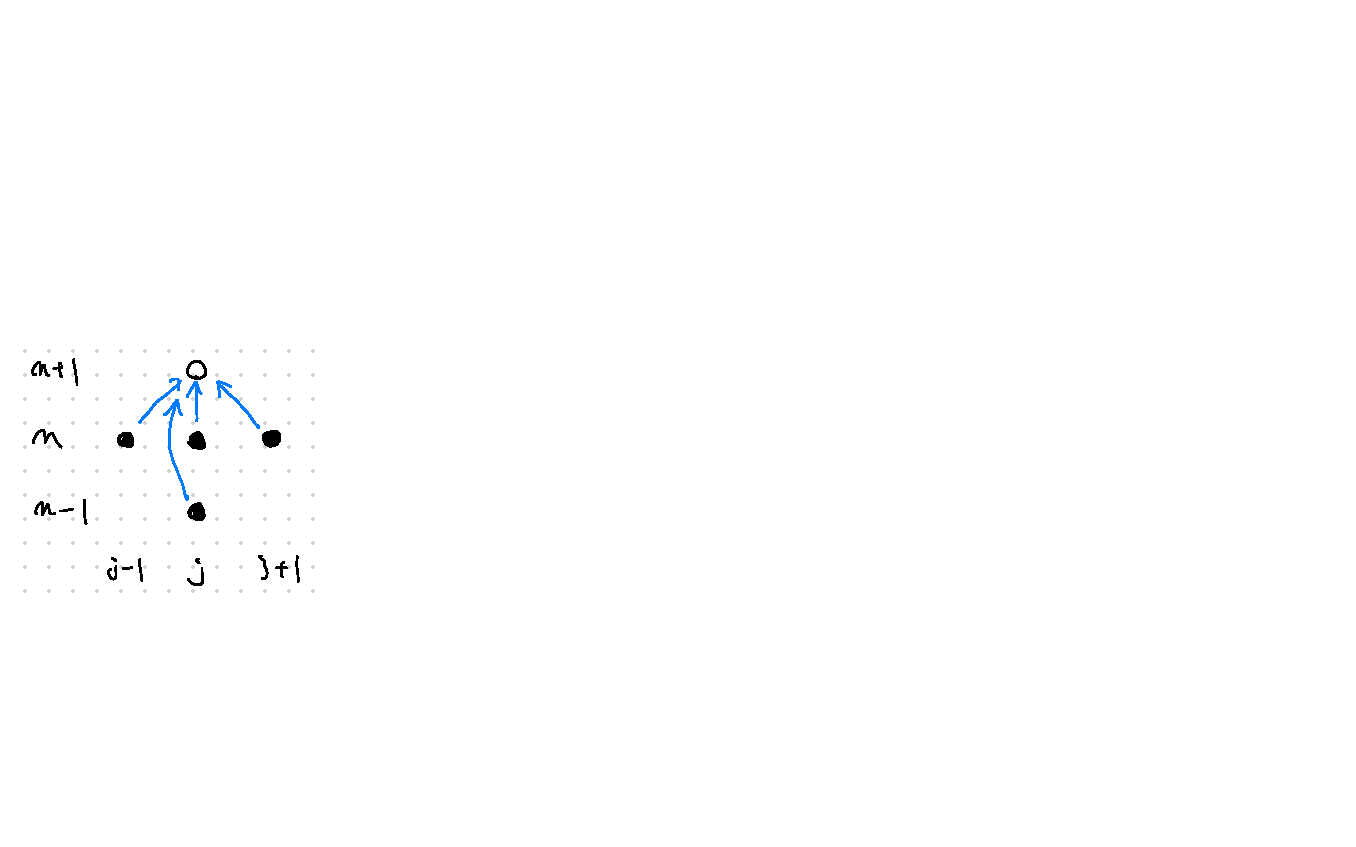
\includegraphics{image/ftcs-2.pdf}}
    \end{center}
  \item 初期条件
    \[
    u_j^0 = f(j\Delta x) \ \ (j=0,1,\cdots,N)
    \]
    初期速度については$n=0$に関する中心差分を考えて
    \[
    \frac{u_j^1 - u_j^{-1}}{2 \Delta t} = g_j \ \ \Rightarrow \ \ u_j^1 = u_j^0 + \Delta t g_j + \frac{\alpha^2}{2} (u_{j+1}^{n} - 2 u_{j}^{n} + u_{j-1}^{n})
    \]
  \end{itemize}
\end{frame}
